

% \begin{table}
% 	\begin{minipage}{0.5\linewidth}
% 		\caption{Student Database}
% 		\label{table:student}
% 		\centering

% \begin{tabular}[t]{llc}
% %%%%%% Title row starts here
% % Temporary header Graph would be better! TBD
% \toprule
% \multicolumn{2}{l}{} & mIOU \\
% \midrule
% \multicolumn{2}{l}{Baseline} & 75.79 \\
% \multicolumn{2}{l}{Baseline + SDC} & 76.37 \\
% \multicolumn{2}{l}{Baseline + LID} & 76.37 \\
% \bottomrule
% \end{tabular}
% 	\end{minipage}\hfill
% 	\begin{minipage}{0.45\linewidth}
% 		\centering
% 		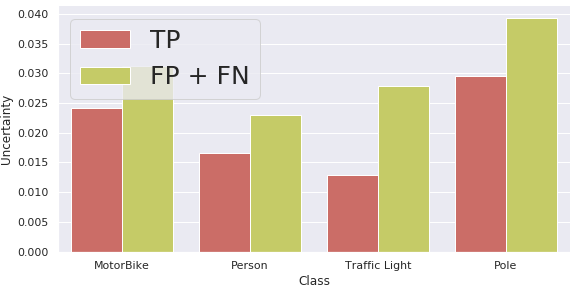
\includegraphics[width=1.0\linewidth]{figures/uncertainty.png}
% 		\captionof{figure}{2-D scatterplot of the Student Database}
% 		\label{ }
% 	\end{minipage}
% \end{table}
\begin{figure}\CenterFloatBoxes
\begin{floatrow}
\ffigbox[1.0\linewidth][]
{%
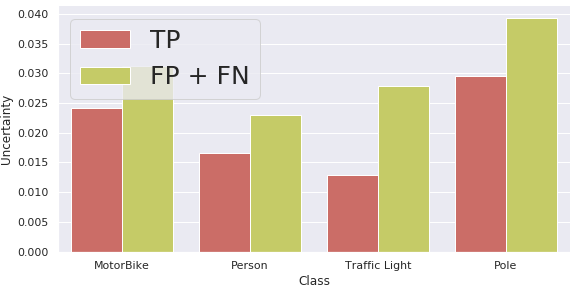
\includegraphics[height=0.4\linewidth]{figures/uncertainty.png}}
{%
\vspace{-0.3em}%
\caption{ Precision vs Recall plot showing uncertainty effectively captures noise in label generation.}\label{fig: figure-label}}
\killfloatstyle\ttabbox[\Xhsize]
{%
\begin{tabular}[b]{llc}
%%%%%% Title row starts here
% Temporary header Graph would be better! TBD
\toprule
\multicolumn{2}{l}{} & mIOU \\
\midrule
\multicolumn{2}{l}{Baseline} & 77.66 \\
\multicolumn{2}{l}{Baseline  + \cite{nvidia_cvpr19} ($\pm 3$)}+ RLL  & 77.24 \\
\multicolumn{2}{l}{Baseline + Ours($\pm 3$)}+ RLL  & 77.50 \\
\bottomrule
\end{tabular}%
}%
{\caption{ Addding a single propagated frame, and relaxed label loss (RLL)~\cite{nvidia_cvpr19} is ineffective.}\label{tab: table-label}}%
\end{floatrow}

% \caption{\small \emph{Left:} The sequence error for SVHN multi-digit recognition
% on crops of $64\times 64$ pixels (64px), and inflated crops of $128 \times 128$
% (128px) which include more background. \textsuperscript{*}The best reported
% result from \cite{Ba14} uses model averagin}
% % }}%
\vspace{-1em}
\end{figure}

% \begin{figure}
% \begin{floatrow}
% \capbtabbox{%
% \centering%
% \begin{tabular}[t]{llc}
% %%%%%% Title row starts here
% % Temporary header Graph would be better! TBD
% \toprule
% \multicolumn{2}{l}{} & mIOU \\
% \midrule
% \multicolumn{2}{l}{Baseline} & 75.79 \\
% \multicolumn{2}{l}{Baseline + SDC} & 76.37 \\
% \multicolumn{2}{l}{Baseline + LID} & 76.37 \\
% \bottomrule
% \end{tabular}
% }{%
%   \caption{This is the great table of asgard}%
% }%
% \ffigbox{%
% \centering%
% 				\label{fig:input-model}
% 				% \centering
% 				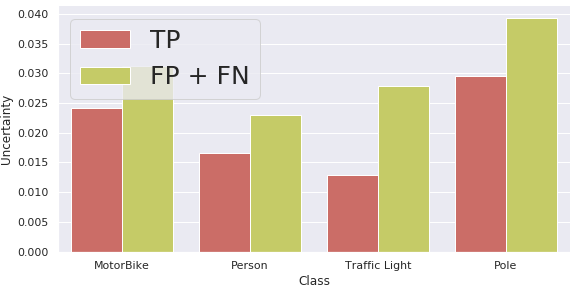
\includegraphics[width=0.5\linewidth]{figures/uncertainty.png}%
% }{%
%   \caption{A figure from asgard}%
% }%
% \end{floatrow}
% \end{figure}



% \begin{figure}[t]
% \begin{center}% \small
% % \setlength{\tabcolsep}{3pt}

% \label{table:svhn}
% 		\subfigure[b]{
% \begin{minipage}{0.45\textwidth}
% \centering
% \begin{tabular}[t]{llc}
% %%%%%% Title row starts here
% \\
% % Temporary header Graph would be better! TBD
% \toprule
% \multicolumn{2}{l}{} & mIOU \\
% \midrule
% \multicolumn{2}{l}{Baseline} & 75.79 \\
% \multicolumn{2}{l}{Baseline + SDC} & 76.37 \\
% \multicolumn{2}{l}{Baseline + LID} & 76.37 \\
% \bottomrule
% \end{tabular}
% \end{minipage}
% % }}%
% \caption{Corrected Evalutation of previous work\cite{nvidia_cvpr19}}
% }
% % \qquad\qquad \qquad\qquad
% % \hspace{2em}
% % \vtop{
% % \hfill
% % \hbox{
% % 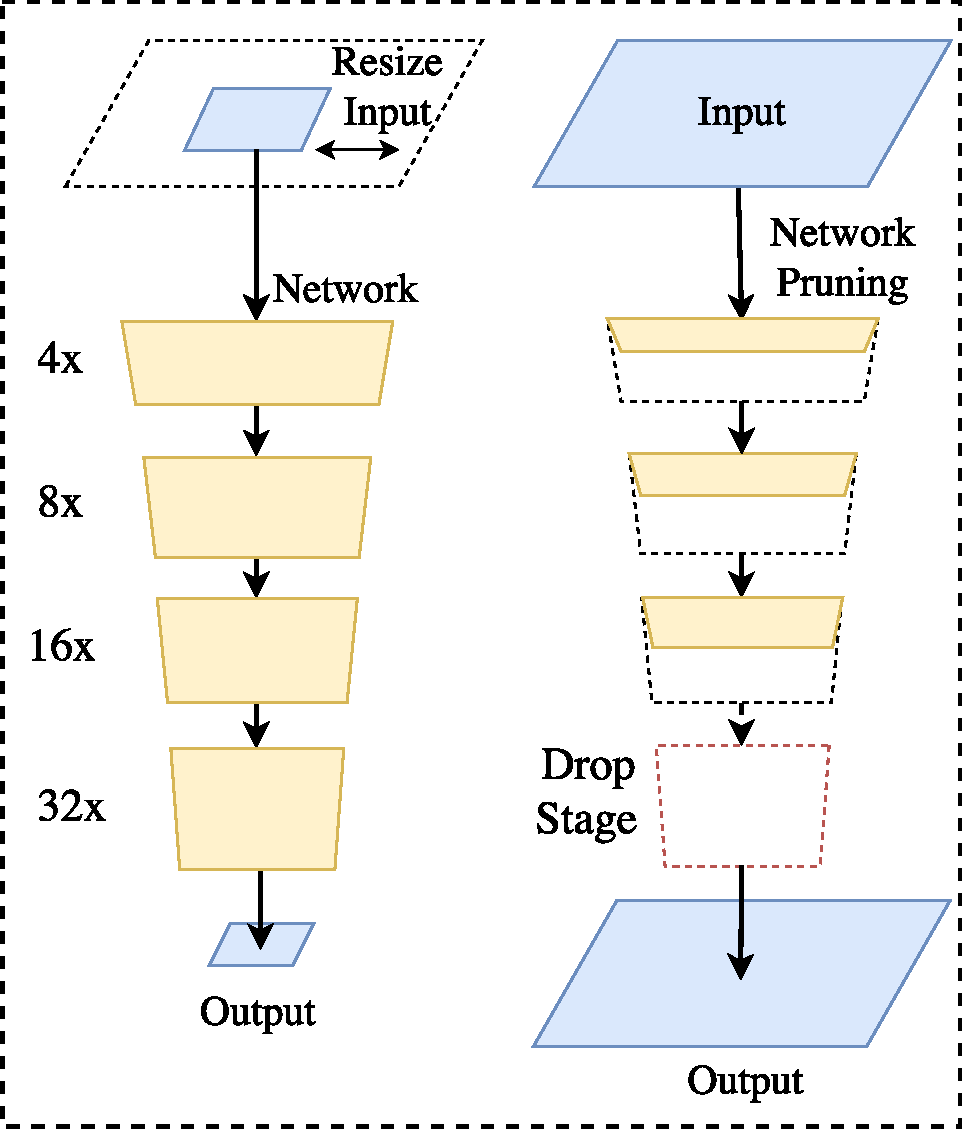
\includegraphics[width=0.6\textwidth]{figures/input_model.pdf}
% 		\subfigure[b]{
% \begin{minipage}{0.30\textwidth}
% \centering
% 				\label{fig:input-model}
% 				% \centering
% 				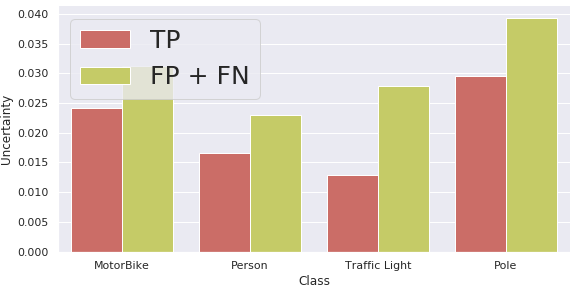
\includegraphics[width=1.0\linewidth]{figures/uncertainty.png}
% \end{minipage}
% \caption{Precision-Recall Curve}
% }

% \caption{\small \emph{Left:} The sequence error for SVHN multi-digit recognition
% on crops of $64\times 64$ pixels (64px), and inflated crops of $128 \times 128$
% (128px) which include more background. \textsuperscript{*}The best reported
% result from \cite{Ba14} uses model averagin}
% % }}%
% \end{center}
% 		\vspace{-2.0em}
% \end{figure}
